\section{Previous Searches} \label{section:higgs_run1results}
On the 4$^{th}$ of July 2012, the two largest experiments at the Large Hadron Collider, ATLAS and CMS, announced an observation of a new particle near the mass of 125 GeV. For that analysis, data collected at proton-proton collisions at $\sqrt{s} = 7$ TeV and $\sqrt{s} = 8$ TeV during the Run 1 production campaign was used. In total, the CMS experiment considered five decay channels: H $\rightarrow$ $\gamma\gamma$, H $\rightarrow$ ZZ, H $\rightarrow$ W$^{+}$W$^{-}$, H $\rightarrow$ $\tau^{+}\tau^{-}$, and H $\rightarrow$ $b\bar{b}$. At the Higgs Boson hypothesis mass of 125.5 GeV, the combined significance of all of the five channels reached 5$\sigma$, which signals the discovery of a new particle near that mass. For the same mass hypothesis, the combination of just the first three channels (H $\rightarrow$ $\gamma\gamma$, H $\rightarrow$ ZZ, H $\rightarrow$ W$^{+}$W$^{-}$) resulted in 5.1$\sigma$ significance of the excess \cite{CMSHiggsRun1Observation}. Higgs decay modes, H $\rightarrow$ $\gamma\gamma$ and H $\rightarrow$ ZZ, are the drivers of the discovery due to the very good mass resolution. Furthermore, the combined measurement of the Higgs Boson mass by ATLAS and CMS experiments in the two most significant decay modes (H $\rightarrow$ $\gamma\gamma$ and H $\rightarrow$ ZZ) was performed and found to be 125.09 GeV \cite{Aad:2015zhl}.

During Run 1 analysis campaign, the decay of the Higgs Boson to two muons has been evaluated. Due to a very low branching fraction of the dimuon decay mode, 0.02\%, which is approximately two orders of magnitude lower than the $\tau\tau$ decay, no excess of events above the expected background around the 125 GeV mass was observed \cite{CMSHiggsRunI}. Therefore, the upper exclusion limits were placed on the production cross section (times branching fraction). Results presented in this search will be further discussed and compared to the Run 1 in Section~\ref{section:higgs_conclusions}. The fact, that an observation of a new particle has been made around the mass of 125 GeV, allows one to significantly narrow down the mass range when searching for the Higgs Boson in a dimuon final state.
 % because the assumption is made that it is the same Higgs Boson that is to be searched for.

% The production of the Higgs Boson at the LHC is dominated by the gluon fusion process with the intermediate top quark loop. At the centre-of-mass energy of $13$ TeV and the hypothesized Higgs Boson mass near $125$ GeV, the production cross-section for this process is one order of magnitude larger than the Vector Boson Fusion (VBF) mode, the next most contributing process. The main feature of the VBF production is the presence of two forward jets in the event going into opposite ends (large separation in pseudo-rapidity coordinate among the two jets) of the CMS detector. The Higgstrahlung or Associated Production, the production of the Higgs Boson in association with either Vector Bosons or $\mathrm{t\bar{t}}$, are the least contributing production processes considered in the search. The full list of the production processes (as CMS datasets) and corresponding cross-sections is provided in the Section~\ref{section:higgs_data}
% \begin{figure}[hbp]
%     \centering
%     \includegraphics[width=0.99\textwidth]{figures/ch_higgs/lhc/lhc_higgs_feynman.jpeg}
%     \caption{Feynman diagrams for the most dominant Higgs Boson production processes at the Large Hadron Collider. Gluon Fusion (a), Vector Boson Fusion (b), Associated Production with Vector Bosons(c), Associated Production with $\mathrm{t\bar{t}}$ (d)}
% \label{fig:higgs_cms_lhc}
% \end{figure}
% The aim of this section is to introduce the LHC Machine and the CMS detector by  briefly reviewing the components that are pertinent to the analysis performed. Very detailed documents outlining the design and architecture of both the CMS and LHC can be found in CMS Technical Design Report \cite{TDR,CMSExperiment} and LHC machine specification \cite{lhcMachine}.

% \subsection{The LHC Machine} \label{subsection:higgs_cms_lhc}
% The Large Hadron Collider (LHC) is a particle accelerating and colliding complex located on the border between France and Switzerland. Figure \ref{fig:higgs_cms_lhc} shows the geographical overview of the location of LHC and of several experiments that are currently hosted there: ATLAS \cite{ATLASExperiment}, CMS, LHCb \cite{LHCbExperiment} and ALICE \cite{ALICEExperiment}. Each of these experiments is located at the beam crossing point along the ring.
% \begin{figure}[hbp]
%     \centering
%     \subfigure[]{
%         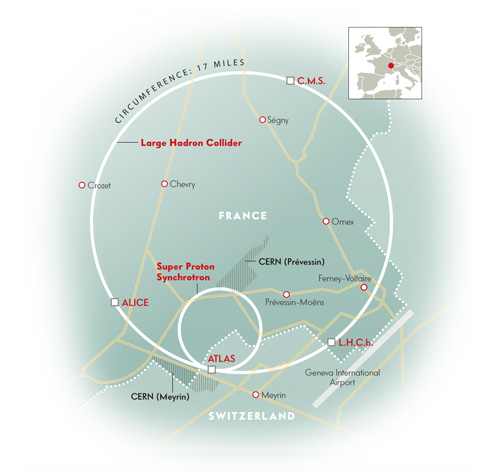
\includegraphics[width=0.99\textwidth]{figures/ch_higgs/misc/lhcring.jpg}
%     }
%     \caption{LHC Accelerator Complex}
%     \label{fig:higgs_cms_lhc}
%  \end{figure}

% The main constituent of the LHC is a 27 km circular tunnel located about 100 m underground and equipped with thousands of various superconducting dipole and quadrupole electromagnets. The operating temperature of the collider electromagnets is about -271\textdegree{}C, which is maintained by a special liquid helium based cryogenic system. Superconducting magnets are used to focus the beam along the ring towards the corresponding interaction points.

% The LHC beams are structured into individual colliding bunches, with ~10$^{11}$ protons per bunch and time separation of 25 ns, which is the period of the proton-proton collisions at the LHC. In total, it is possible to have at most about 3600 bunches, however only up to 2808 could be filled with protons. The rest, called Abort Gap, is used for experiment's maintenance, calibration, or other accelerator-related work.

% \subsection{The CMS Detector} \label{subsection:higgs_cms_generaldescription}
% The Compact Muon Solenoid, one of the two largest experiments hosted at the LHC, is a two-fold creature; first of all, it is a one of its kind general purpose particle detector system, which consists of multiple components and whose primary objective is to record and reconstruct physics events that could help study the fundamental building blocks of nature. It acts like a camera, recording the footprint of the physics interactions which particle physicists use to deduce the underlying physics. The Compact Muon Solenoid is also an experiment, a collaboration of thousands of people whose combined effort made it possible to build and operate such a device. From people involved in data-taking at Point 5 and detector maintainance experts to people performing the analysis of recorded events and making sure that thecollected data is of the highest quality - it is one of the best examples when group effort produces results of highest esteem.

% The most important component of CMS that makes it stand out among other experiments is the superconducting solenoid with magnetic field of 3.8 T. The magnet is located just outside of the HCAL subsystem and plays a crucial role in the overall architecture of CMS. In particular, due to the strength of magnetic field, significant improvements are expected in the search for the Higgs Boson decaying via two muons due to a high resolution of the muon system together with the power of the magnet. The closest subsystem of CMS to the interaction point is the Silicon Tracker \cite{Tracker}, whose primary objective is to measure the momentum of the charged particles passsing through. What follows are Electromagnetic \cite{ECAL} and Hadronic \cite{HCAL} subsystems which respectively consist of several subdetectors with varying performance characteristics. Muon Systems are located just outside of the magnet and comprise different technologies depending on the $\eta$ location \cite{Muon}.

% The Large Hadron Collider is not merely a challenging project from an engineering standpoint, it is also a data factory, one of its kind, that presents a unique challenge for the data processing and analysis domain. The amount of data that gets generated quickly becomes unmanagable and one has to be careful when selecting what to preserve and what to abandon. The collision rate is 40 MHz and the compressed size of just one event coming from CMS is on the order of 1 KB. That amounts to 40 GB/s and extrapolating up to a single hour of datataking it is at the order of 140 TB/h - obviously this becomes unfeasible very quickly. For the purpose of selection of events of interest, all HEP Experiments employ a sophisticated Trigger System, whose purpose is to select the physics events of interest. CMS has two layers for event triggering: Level 1 \cite{L1Trigger} and High Level Trigger (HLT) \cite{HLTrigger}. Level 1 trigger system is a hardware based processing system, that is tightly integrated with the rest of the subsystems' electronics. Level 1 allows CMS to reduce the event rate from 40 MHz down to 100 KHz. This is achieved by applying basic selections at hardware level (integration with the subsystems' electronics results in zero copy processing) using reduced content information known as Trigger Primitives (TPs).

% The 100 KHz output of Hardware Trigger System gets further reduced by the High Level Trigger system, down to 1 KHz that gets actually written to disk. This content reduction is achieved by employing high level information produced via the reconstruction procedure. CMS High Level Trigger System is a reasonable-sized High Perfomance Cluster (HPC) Complex which takes the output of Level 1 and acts as a filtering farm, preserving only events that should be stored to disk for offline processing. The software framework that gets used is the same one as for offline data analysis, however certain reconstruction steps are optimized for performance.

% %\subsection{Tracker System} \label{subsection:higgs_cms_tracker}
% %Explain Pixels and Tracker

% %\subsection{Electromagnetic Calorimeter} \label{subsection:higgs_cms_em}
% %Electromagnetic Calorimeter (or Ecal for breivity) is a subsystem of CMS with the primary objective to

% %\subsection{Hadronic Calorimeter} \label{subsection:higgs_cms_hcal}
% %Hadron Calorimeter (or Hcal for breivity) is a subsystem of CMS with the primary objective to identify and measure energy of jets. It consists of four separate parts: Hadron Barrel, Hadron Endcap, Hadron Outer and Hadron Forward.

% %\subsection{Muon System} \label{subsection:higgs_cms_muon}
% %Describe the Muon Systems

% %\subsection{Trigger System} \label{subsection:higgs_cms_trigger}

% %\subsection{Data Acquisition Software}

% %\subsection{Data Analysis Software} \label{subsection:higgs_cms_cmssw}
% %Describe the Software for Analysis